\let\counterwithout\relax
\let\counterwithin\relax
\documentclass[final]{fhnwreport}       %[mode] = draft or final
\usepackage{color, colortbl}
\usepackage{rotating, rotfloat,ragged2e, hyphenat, diagbox, wrapfig}
\definecolor{grau}{gray}{0.9}
\definecolor{hellgrau}{gray}{0.95}

                                        %{class} = fhnwreport, article, 
                                        %          report, book, beamer, standalone
%%---Main Packages-----------------------------------------------------------------------
\usepackage[english, ngerman]{babel}	%Mul­tilin­gual sup­port for LaTeX
\usepackage[T1]{fontenc}				%Stan­dard pack­age for se­lect­ing font en­cod­ings
\usepackage[utf8]{inputenc}				%Ac­cept dif­fer­ent in­put en­cod­ings
\usepackage{lmodern}                    %The newer Font-Set
\usepackage{textcomp}					%LaTeX sup­port for the Text Com­pan­ion fonts
\usepackage{graphicx} 					%En­hanced sup­port for graph­ics
\usepackage{float}						%Im­proved in­ter­face for float­ing ob­jects
\usepackage{ifdraft}                    %Let you check if the doc is in draft mode

%%---Useful Packages---------------------------------------------------------------------
\usepackage[pdftex,dvipsnames]{xcolor}  %Driver-in­de­pen­dent color ex­ten­sions for LaTeX
\usepackage{csquotes}                   %Simpler quoting with \enquote{}
\usepackage{siunitx} 					%A com­pre­hen­sive (SI) units pack­age
\usepackage{listings}					%Type­set source code list­ings us­ing LaTeX
\usepackage[bottom]{footmisc}			%A range of foot­note op­tions
\usepackage{footnote}					%Im­prove on LaTeX's foot­note han­dling
\usepackage{verbatim}					%Reim­ple­men­ta­tion of and ex­ten­sions to LaTeX ver­ba­tim
\usepackage[textsize=footnotesize]{todonotes} %Mark­ing things to do in a LaTeX doc­u­ment

%%---Tikz Packages-----------------------------------------------------------------------
\usepackage{standalone}
\usepackage{tikz}
\usepackage{circuitikz}
\usetikzlibrary{arrows}
\usetikzlibrary{calc}
\usetikzlibrary{intersections}

%%---Math Packages-----------------------------------------------------------------------
\usepackage{amsmath}					%AMS math­e­mat­i­cal fa­cil­i­ties for LaTeX
%\usepackage{amssymb}					%Type­set­ting symbols (AMS style)
%\usepackage{array}						%Ex­tend­ing the ar­ray and tab­u­lar en­vi­ron­ments
%\usepackage{amsthm}					%Type­set­ting the­o­rems (AMS style)

%%---Table Packages----------------------------------------------------------------------
\usepackage{tabularx}					%Tab­u­lars with ad­justable-width columns
%\usepackage{longtable}
\usepackage{multirow}					%Create tab­u­lar cells span­ning mul­ti­ple rows
\usepackage{multicol}					%In­ter­mix sin­gle and mul­ti­ple columns

%%---PDF / Figure Packages---------------------------------------------------------------
\usepackage{pdfpages}					%In­clude PDF doc­u­ments in LaTeX
\usepackage{pdflscape}					%Make land­scape pages dis­play as land­scape
\usepackage{subfig}					    %Fig­ures di­vided into sub­fig­ures

%%---Other Packages----------------------------------------------------------------------
%\usepackage{xargs}                     %De­fine com­mands with many op­tional ar­gu­ments

%%---Bibliography------------------------------------------------------------------------
\usepackage[style=ieee,urldate=comp,backend=biber]{biblatex}
\addbibresource{literature/bibliography.bib}

%%---Main Settings-----------------------------------------------------------------------
\graphicspath{{./graphics/}}			%Defines the graphicspath
%\geometry{twoside=false}				    %twoside=false disables the "bookstyle"
\setlength{\marginparwidth}{2cm}
\overfullrule=5em						%Creates a black rule if text goes over the margins => debugging


%%---User Definitions--------------------------------------------------------------------
%%Tabel-Definitions: (requires \usepackage{tabularx})
\newcolumntype{L}[1]{>{\raggedright\arraybackslash}p{#1}}    %column-width and alignment
\newcolumntype{C}[1]{>{\centering\arraybackslash}p{#1}}
\newcolumntype{R}[1]{>{\raggedleft\arraybackslash}p{#1}}

%%---Optional Package Settings-----------------------------------------------------------
%Listings-Settings: (requires \usepackage{listings}) => Example with Matlab Code
\lstset{language=Matlab,%
    basicstyle=\footnotesize\ttfamily,
    breaklines=false,%
    morekeywords={switch, case, otherwise},
    keywordstyle=\color{Blue},%
    tabsize=2,
    %morekeywords=[2]{1}, keywordstyle=[2]{\color{black}},
    identifierstyle=\color{Black},%
    stringstyle=\color{Purple},
    commentstyle=\color{Green},%
    showstringspaces=false,%without this there will be a symbol in the places where there is a space
    numbers=left,%
    numberstyle={\tiny \color{black}},% size of the numbers
    numbersep=9pt, % this defines how far the numbers are from the text
    %emph=[1]{word1, word2,...},emphstyle=[1]\color{red}
}							
			                %loads all packages, definitions and settings												
\title{«DJ» EMI Filter für Schaltnetzteil}          			%Project Title
\author{Fachbericht}  		%Document Type => Technical Report, ...
\date{Windisch, 20.04.2019}             		%Place and Date

\begin{document}

%%---TITLEPAGE---------------------------------------------------------------------------
\selectlanguage{ngerman}                %ngerman or english
\maketitle

\vspace*{-1cm}						    %compensates the space after the date line.
\vfill
\begin{figure}[H]
\centering
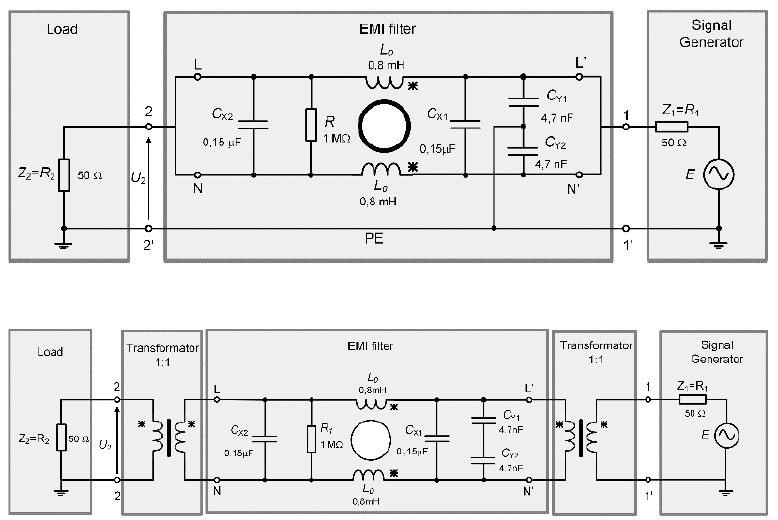
\includegraphics[width=10cm]{titelBild.png}
\end{figure}
\vfill

{
\renewcommand\arraystretch{2}
\begin{center}
\begin{tabular}{ >{\bf} l p{10cm} l }
Hochschule&Hochschule für Technik - FHNW\\
Studiengang&Elektro- und Informationstechnik\\
Auftraggeber&Dr. Luca Dalessandro\\
Betreuer&Prof. Dr. Sebastian Gaulocher \newline Prof. Peter Niklaus \newline Prof. Dr. Richard Gut \newline  Dr. Anita Gertiser \newline Pascal Buchschacher \\
Autoren&\textbf{Gruppe 1} \newline Niklaus Schwegler \newline Lukas von Däniken \newline Pascal Puschmann  \newline Simon Rohrer \newline Marco Binder\\
Version&2.0 %Normally not used!
\end{tabular}
\end{center}
}

\clearpage

%\selectlanguage{ngerman}				%ngerman or english
\thispagestyle{empty}
			
%%---TABLE OF CONTENTS-------------------------------------------------------------------
\pagenumbering{Roman}		
%\selectlanguage{ngerman}				%ngerman or english
\tableofcontents
\clearpage

%%---TEXT--------------------------------------------------------------------------------
\pagenumbering{arabic}
\section{Abstract} \label{sec:abstract}


\section{Einleitung} \label{sec:einleitung}
Entwurf Einleitung P2 EMI-Filter Team 1

Gemäss des Lastenhefts wurde der Auftrag erteilt, eine Simulationssoftware zu entwickeln. Diese Simulationssoftware soll die Einfügedämpfung eines EMI-Filters simulieren und grafisch darstellen. EMI-Filter werden üblicherweise in Schaltnetzteile verbaut, um zu verhindern, dass Störungen zurück ins Netz gespeist werden. Netzgeräte können unter Umständen hohe Frequenzen erzeugen, die sich nicht gut mit der Netzfrequenz von 50 Hz vertragen. Der EMI-Filter filtert genau diese hochfrequenten Signale heraus, um zu verhindern, dass andere Geräte, die auch ans Netz angeschlossen werden, nicht davon beeinträchtigt werden.

Um die Einfügedämpfung zu ermitteln, soll das EMI-Filter bezüglich der Gleich- und Gegentaktschaltung untersucht werden. Dies geschieht anhand zweier Funktionen für Gleich- und Gegentaktschaltung. Die Funktionen zeigen die Einfügdämpfung für einen Frequenzbereich bis 30MHz.Die beiden Schaltungen beinhalten die parasitären Parameter der elektrischen Komponenten, sodass eine möglichst wahrheitsgetreue Simulation gemacht werden kann. Die entwickelte Software soll die Einfügedämpfung grafisch darstellen.  Die Resultate werden für die Gleich- und Gegentaktschaltung in separaten Funktionen dargestellt. Des Weiteren sollen die elektrischen Komponenten der Schaltungen in der Simulationssoftware variiert werden können.
 
Damit sichergestellt werden kann, dass die Simulationen mathematisch korrekt sind, werden alle Berechnungen zuerst in MATLAB durchgerechnet. Diese Ergebnisse werden mit Simulationen der Simulationssoftware MPLAB MINDI verglichen. Des Weiteren wird überprüft, wie die Schaltung vereinfacht werden kann. Dies erfolgt einerseits durch Symmetrien der Schaltung, was dazu führt, dass Komponenten zusammengefasst werden können. Andererseits auch durch Weglassen aufgrund von vernachlässigbarem Einfluss auf die Simulationen. Die Softwarestruktur orientiert sich am gängigen Prinzip der MVC(Model-View-Control). Diese Strukturierung begünstigt einen modularen Aufbau, was die Software einfach erweiterbar macht und zudem eine unkomplizierte Wartung ermöglicht. Des Weiteren wird die Software anhand des Testkonzepts Modul für Modul getestet.

Im Fokus des Fachberichts befindet sich die Software, da das zu entwickelnde Produkt eine Simulationssoftware ist. Der Fachbericht ist nach dem Top-Down-Prinzip aufgebaut. In einem ersten Schritt wird die Software als Ganzes Beschrieben. In den darauffolgenden Kapiteln befinden sich die Dokumentationen der beiden Teile der Software. Die Software wird aufgegliedert in den Teil Benutzeroberfläche und den Teil Ermittlung der Einfügedämpfung. Um den Fachbericht schlank zu gestalten, werden sämtliche theoretische Grundlagen im Anhang platziert. Falls in Kapiteln entsprechende Theorie wichtig ist wird darauf verwiesen.


\section{Software} \label{sec:software}

knackiger Top-Down beschrieb des IST-Zustands der fertigen software. 

Es werden stets Fachbegriffe verwendet. 


In dieser Section wird erklärt warum die Software wie aufgebaut ist.

Ebenfalls wird beschrieben welche berechnungen in welcher Klasse durchgeführt werden
Das heisst, dass wir hier auch Bilder der Vereinfachten Schaltung zeigen und wie wir diese Aufteilen in einzelne Glieder


\section{Testkonzept}\label{sec:testkonzept}
Wieso, weshalb und Warum
\subsection{Prinzip} \label{prinzip}
Wie ist das Testkonzept aufgebaut
\subsection{Validierung} \label{validierung}
Testergebnisse darstellen und Interpretieren

Ebenfalls wird hier beschrieben welche Werte wir mit der Simulation und mit Matlab erreicht haben

\section{Schluss} \label{sec:schluss}
Zum Abschluss des Projektes und nachdem alle Test durchgeführt wurden, wird die Software dem Auftraggeber zur Verfügung gestellt. Alle im Pflichtenheft gesteckte Muss-Ziele wurden zufriedenstellend umgesetzt. Die Software ist in der Lage die Eifügedämpfung eines EMI-Filters grafisch darzustellen. Ausserdem ist es möglich verschiedene Filterprofile anzulegen und sie zu speichern. Die verschieden Filter können gleichzeitig im Plot angezeigt werden. 

Die grösste Herausforderung während des Projektes bestand aus der Erarbeitung der elektrotechnischen Grundlagen und die Berechnung der Einfügedämpfung des Netzwerkes in DM und CM. Die Entwicklung des Softwaregrundgerüsts ging zügig vorwärts. Die Schwierigkeiten bei der Software waren beispielsweise die Implementierung der durchgeführten Berechnungen in den Code und die Verarbeitung der Werte, die in die GUI eingegeben werden. Um die Performence nicht einzuschränken, können nur 10 Filterprofile gleichzeitig angezeigt werden.

Schlussendlich konnten alle Schwierigkeiten gut gemeistert werden. Die Software könnte natürlich noch weiterentwickelt werden.  Eine weitere sinnvolle Funktion wäre eine Monte-Carlo Analyse. Diese wurde jedoch aus Zeitgründen nicht implementiert. Als abschliessendes Fazit ist zu sagen, dass dieses Projekt erfolgreich und termingerecht durchgeführt werden konnte. 



%%---BIBLIOGRAPHY------------------------------------------------------------------------

{\sloppypar
\selectlanguage{ngerman}	
\setlength{\bibitemsep}{\baselineskip}
\printbibliography[heading=bibintoc]
\label{sec:lit}
}

%%---Anhang------------------------------------------------------------------------

\section{Anhang} \label{sec:anhang}



\subsection{Testkonzept} \label{subsec:eltech}
\begin{figure}[H]
	\centering
	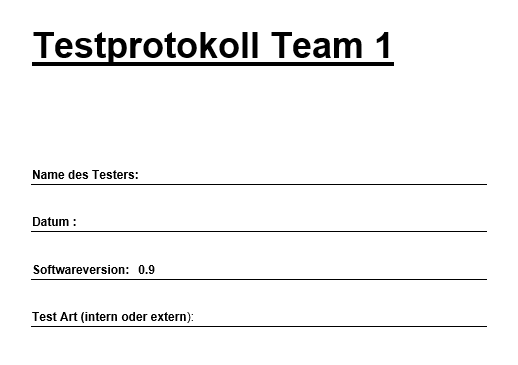
\includegraphics[width=16cm]{Protokoll.png}
	\label{fig:Protokoll}
\end{figure}

\begin{figure}[H]
	\centering
	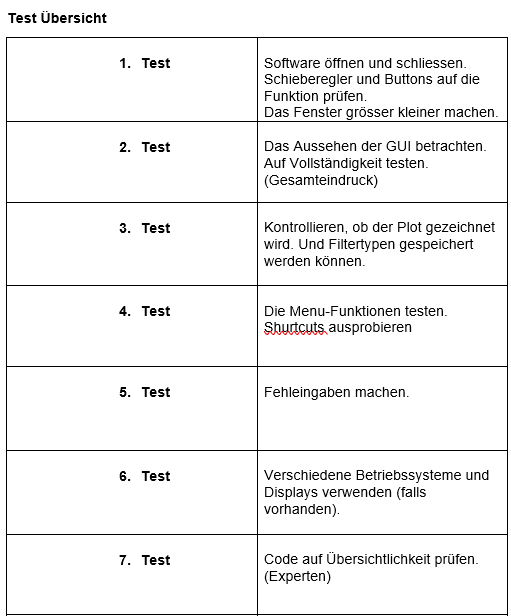
\includegraphics[width=16cm]{uebersicht.png}
	\label{fig:übersicht}
\end{figure}

\begin{figure}[H]
	\centering
	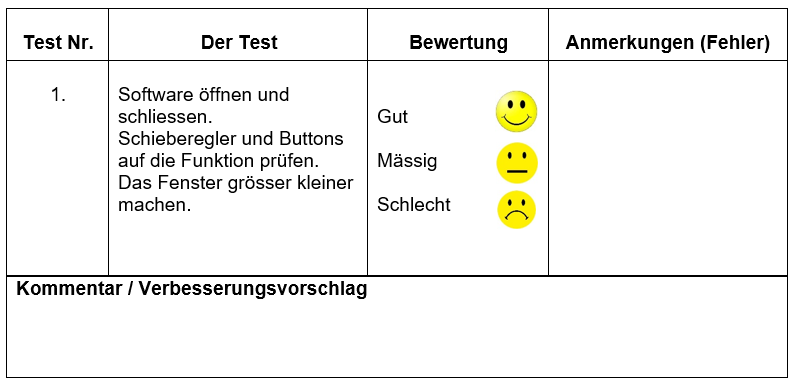
\includegraphics[width=16cm]{Test1.png}
	\label{fig:Test1}
\end{figure}

\begin{figure}[H]
	\centering
	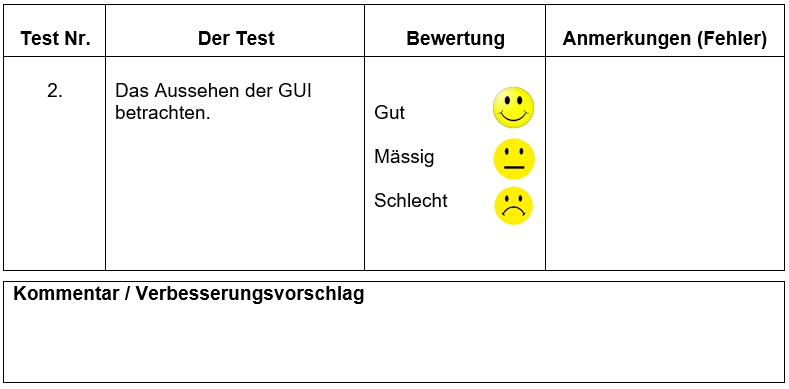
\includegraphics[width=16cm]{Test2.png}
	\label{fig:Test2}
\end{figure}

\begin{figure}[H]
	\centering
	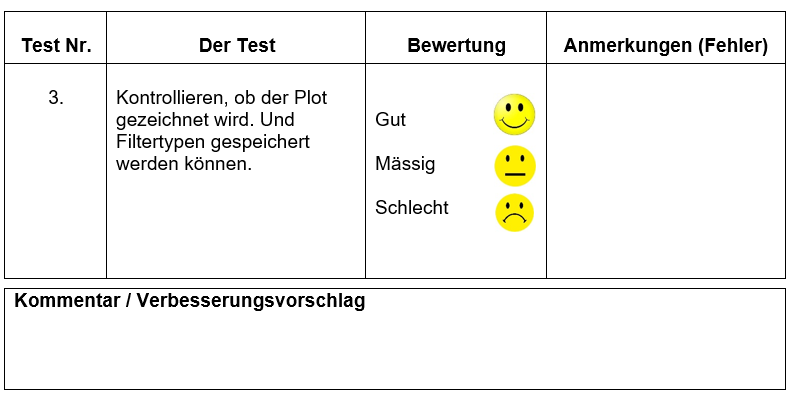
\includegraphics[width=16cm]{Test3.png}
	\label{fig:Test3}
\end{figure}

\begin{figure}[H]
	\centering
	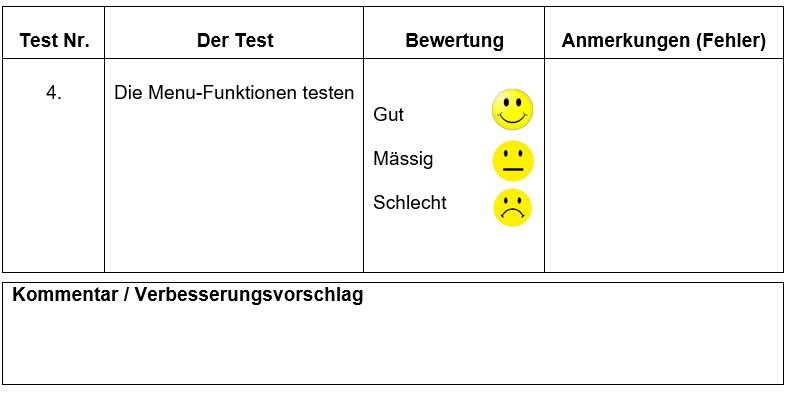
\includegraphics[width=16cm]{Test4.png}
	\label{fig:Test4}
\end{figure}

\begin{figure}[H]
	\centering
	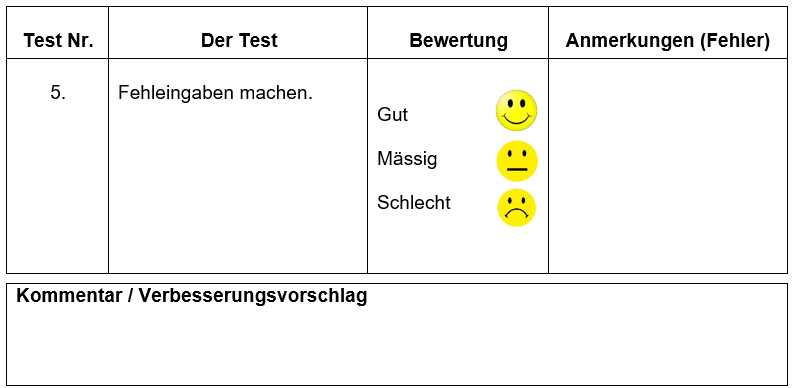
\includegraphics[width=16cm]{Test5.png}
	\label{fig:Test5}
\end{figure}

\begin{figure}[H]
	\centering
	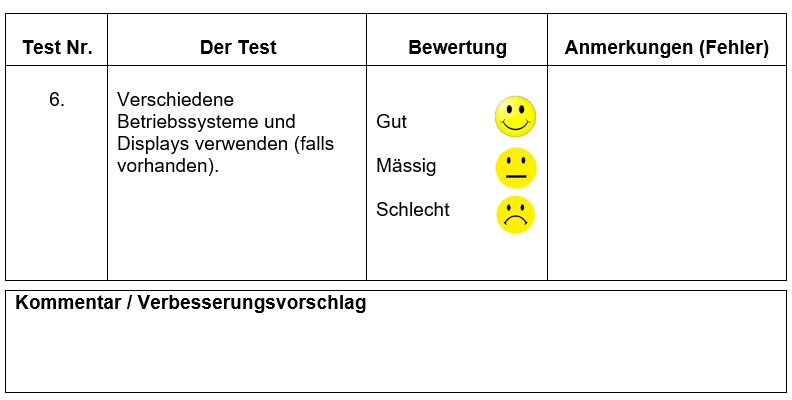
\includegraphics[width=16cm]{Test6.png}
	\label{fig:Test6}
\end{figure}

\begin{figure}[H]
	\centering
	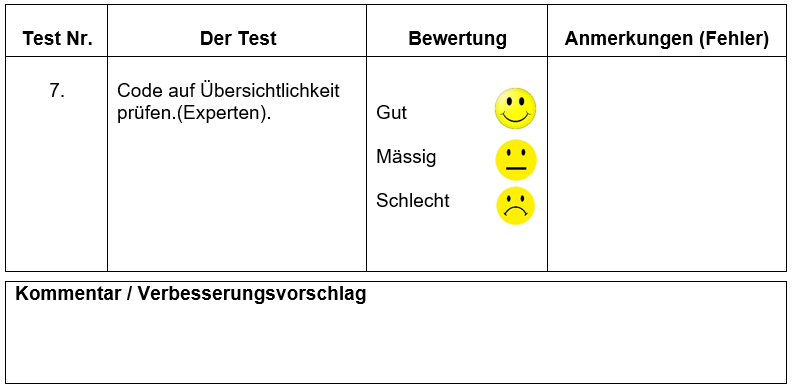
\includegraphics[width=16cm]{Test7.png}
	\label{fig:Test7}
\end{figure}

\begin{figure}[H]
	\centering
	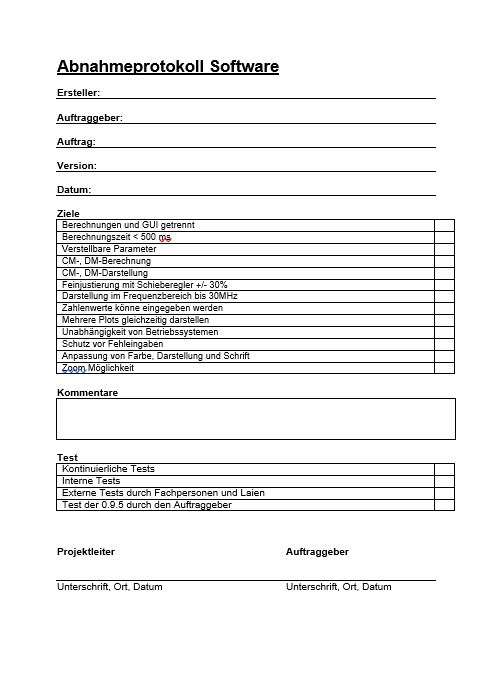
\includegraphics[width=16cm]{Abnahme.png}
	\label{fig:Protokoll}
\end{figure}

%%---NOTES for DEBUG---------------------------------------------------------------------
\ifdraft{%Do this only if mode=draft
%%requires \usepackage{todonotes})
\newpage
\listoftodos[\section{Todo-Notes}]
\clearpage
}
{%Do this only if mode=final
}
\end{document}
